\documentclass[11pt]{article}
\usepackage[margin=1in]{geometry}
\usepackage{booktabs}
\usepackage{graphicx}
\usepackage{amsmath}
\usepackage{hyperref}
\usepackage{xcolor}
\title{\textbf{Removing the VDM: 3D-Tracking Geometric State Judgment\\
for Code-as-Policies Robot Agents}}
\author{cap-x-se / track-judge experiment}
\date{\today \quad\textcolor{gray}{\small(living draft --- figures/tables auto-generated by \texttt{make\_figs.py})}}

\begin{document}
\maketitle

\begin{abstract}
Agentic Code-as-Policies systems call a Visual Differencing Model (VDM)---a VLM---every turn
to judge task state and steer the agent's self-correction. We argue the VDM is a
\emph{redundant LLM call}: a second VLM invocation whose errors are correlated with the policy
LLM, returning largely the agent's own opinion at real latency and cost. We \emph{remove} it
and introduce a \emph{self-evaluating} agent that self-plans \emph{and} self-evaluates---both
as code, with \emph{no LLM call} at judgment time and free use of any packages---basing its
state judgment on agent-written geometric code over \emph{3D point trajectories} (TAPIP3D), a
decorrelated, physically grounded, local signal. On libero-pro with a single Gemini
cap-agent0, we test whether this makes the agent both more successful and faster.
\textbf{[Result: TBD --- this is a living draft.]}
\end{abstract}

\section{Introduction}
The per-turn VDM in cap-x-se is an extra VLM call. Because it shares the policy LLM's modality
and family, its judgments are correlated with the policy's own beliefs, so it adds little
\emph{independent} information while costing a full inference each turn. We ask whether the VDM
can be removed entirely and replaced with a fundamentally different signal: deterministic
geometry over the 3D trajectories of tracked scene points. The agent, given the same initial
static frame, writes \emph{two} artifacts---execution code and a state-judgment function; the
latter runs on the dense RGB-D rollout video through a 3D point tracker and decides
progress/done/failure geometrically. Our thesis is that this is \textbf{both faster}
(no per-turn VLM; early abort on geometric failure) \textbf{and more successful} (a richer,
grounded, decorrelated signal).

\section{Why a 3D trajectory beats a frame-diff VLM}
\label{sec:why}
A VDM returns a discrete 2D semantic snapshot; a tracker returns continuous metric 3D
trajectories of chosen masks. The latter affords judgments the VDM structurally cannot make:
\begin{itemize}\itemsep2pt
  \item \textbf{Collision / near-miss}: minimum inter-object distance over time (cm).
  \item \textbf{Grasp slip}: object points tracked \emph{relative to the gripper}; loss of
        co-motion $\Rightarrow$ slip, caught mid-motion.
  \item \textbf{Early failure $\to$ early abort}: detect failure during execution, retry
        immediately (primary speed and success lever).
  \item \textbf{Drop detection}: descent past support height $+$ free-fall signature.
  \item \textbf{3D containment / placement}: points entering the target container's 3D volume,
        persistent across the last $K$ frames.
  \item \textbf{Occlusion robustness}: occluded points' positions are predicted by the tracker.
  \item \textbf{Appearance/viewpoint invariance}; \textbf{multi-object relations}
        (on-top-of, inside, aligned); \textbf{determinism/debuggability};
        \textbf{dense, cheap, graded progress}; ``right motion, wrong outcome'' (missed grasp).
\end{itemize}

\section{Method}
\textbf{Agent.} cap-agent0: a single-LLM (Gemini) Code-as-Policies loop that writes Python
executed against bound robot APIs, with multi-turn REGENERATE/FINISH self-correction.
\textbf{Arm A (baseline):} the stock VDM. \textbf{Arm B (treatment):} VDM removed; per-turn
feedback comes from the agent-written geometric judge over TAPIP3D 3D tracks (\S\ref{sec:why}),
which selects its own masks. The two arms differ only in the feedback mechanism (a single
config switch); the agent, LLM, suites, seeds and init states are identical.

\textbf{Tracking judge.} The rollout is recorded as a dense RGB-D video with known camera
intrinsics/extrinsics (exact in simulation); per turn it is tracked to 3D point trajectories in
the world frame, and the agent's judge function applies geometric primitives to emit
\{progress, done, failure, abort\}. All tracking is visualized and saved for debugging.

\section{Experimental setup}
\textbf{Benchmark:} libero-pro; success is ground-truth \texttt{check\_success()}. A dev subset
is used to iterate; $\geq 2$ suites are held out for generalisation and never tuned on.
\textbf{Metrics:} task success rate and median wall-clock per task, reported together.
\textbf{Protocol:} an autonomous self-evolve loop optimises Arm B; the win condition is to beat
Arm A on \emph{both} metrics. Arm B is scored as the pure method (no VDM/ground-truth backstop).

\section{Results}
\emph{Living section --- regenerated on every accepted generation.}

\begin{table}[h]\centering
\caption{Headline: VDM baseline (A) vs.\ tracking with the VDM removed (B), dev suites.}
% AUTO-GENERATED by make_figs.py — do not edit by hand.
\begin{tabular}{lrr}
\toprule
metric & VDM (A) & tracking (B) \\
\midrule
success rate & -- & -- \\
median task time (s) & -- & -- \\
judge latency / turn (s) & -- & -- \\
VLM calls / turn & -- & -- \\
\bottomrule
\end{tabular}

\end{table}

\begin{figure}[h]\centering
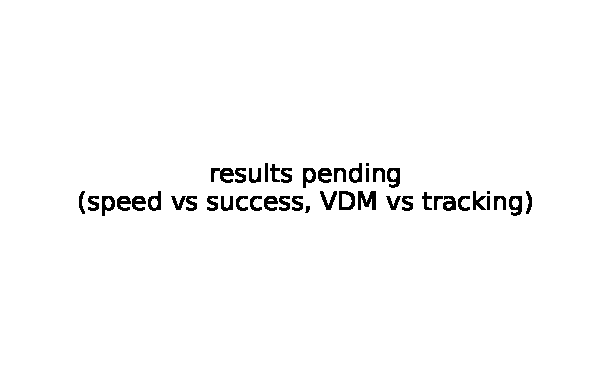
\includegraphics[width=0.62\linewidth]{fig_tradeoff.pdf}
\caption{Speed vs.\ success. Target: B upper-left of A (faster and more successful).}
\end{figure}

\begin{table}[h]\centering
\caption{Per-suite success and speed (dev + held-out).}
% AUTO-GENERATED by make_figs.py — do not edit by hand.
\begin{tabular}{lcccc}
\toprule
suite & A succ & B succ & A time & B time \\
\midrule
\multicolumn{5}{c}{\emph{results pending}} \\
\bottomrule
\end{tabular}

\end{table}

\begin{figure}[h]\centering
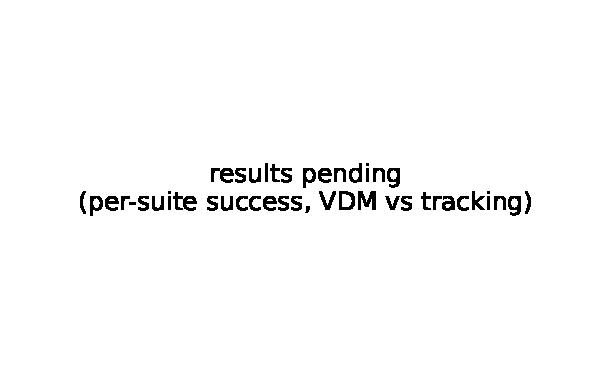
\includegraphics[width=0.85\linewidth]{fig_per_suite.pdf}
\caption{Per-suite success rate, VDM (A) vs.\ tracking (B).}
\end{figure}

\section{Discussion}
\textbf{[TBD.]} Mechanism evidence (\S\ref{sec:why}): which capabilities drive accepted gains,
and an ablation isolating early-abort (speed) from the richer signal (success). The
decorrelation claim---that geometry supplies information the correlated VDM does not---should be
substantiated by cases where the tracker catches failures the VDM misses.

\section{Limitations}
The tracker is not real-time ($\sim$1--2.5\,fps); per-turn judge cost must still net out faster
than a VLM call (early abort is the lever). Simulation depth is exact; a real-robot port is
noisier (results here are a sim upper bound). Judge quality is bounded by mask quality. Wins
must come from transferable geometric principles, checked on held-out suites.

\section{Conclusion}
\textbf{[TBD]} --- does removing the VDM, replaced by 3D-tracking geometric judgment, improve
both success and speed?

\end{document}
